\section{Introduction}
\label{sec:intro} 
Estimation of hands and objects is fundamental and crucial for understanding meaningful interpretation of human action and
behaviour. It provides enormous knowledge for environmental perception and teaching manipulating systems. With the advent of deep learning, pose estimation tasks have significantly made progress such as RGB-based \cite{cai20203d, zimmermann2017learning, gao2019variational, xiang2017posecnn, tremblay2018deep}, depth-based \cite{oberweger2017deepprior++, moon2018v2v, xiong2019a2j, ge20173d, cai2022ove6d, li2020category}, and RGB-D methods \cite{kazakos2018fusion, yuan20193d}. Jointly estimation of hands objects under interaction, however, has attracted less attention due to chronic challenges. This requires simultaneously predicting the pose and shape of hands and objects during the hands handling and executing the objects. In this paper, we propose a novel network to tackle this problem from RGB-D images. 

\begin{figure}[t]
\center
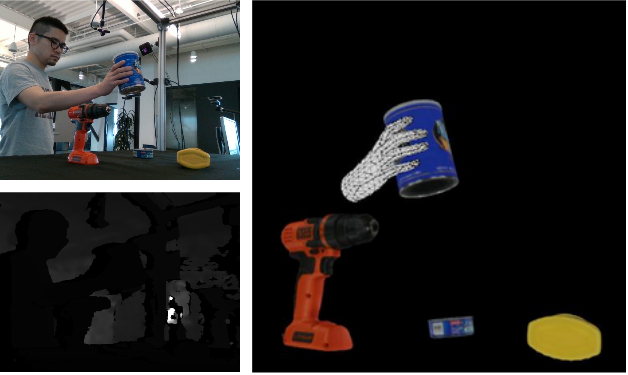
\includegraphics[width=\linewidth]{Figs/result_exp.png}
\label{fig:result_exp}
\caption{Example of RGB-D.}
\end{figure}

Joint hand-object pose estimation under interaction, on the other hand, is a much more challenging problem. The hand shape is notorious for being self-occlusion. This problem is adversely serious in the context when the hand manipulating an object. The naive approach is estimating the shape of the hands and objects seperately. Such methods leverage the success of object pose estimation and hand shape reconstruction independently without considering the correlations between themselves. They totally ignore the heavily dependencies of hand pose on the held object's shape, and and vice versa. Intuitively, the presence of object strongly defines and constrains the hand grasps and therefore limits the feasible hand gestures to a restricted number. Similarly, determining hand gestures provides a cue for estimating the shape and pose of the held object. Consequently, simultaneously predicting the shapes of both hand and object soonly catches the attention of computer vision researchers. 

Inspired by the above perspective, some deep learning-based methods \cite{hasson2019learning, hasson2020leveraging, tekin2019h+, tse2022collaborative, liu2021semi, oikonomidis2011full, lu2021understanding, hasson2021towards, wang2020learning} joinly learn the hand and object poses from a single RGB image. Whereas, \cite{choi2017robust, zhang2021single, goudie20173d, oberweger2019generalized} focus on another input format, depth images, to achieve the expected results. However, they pose a threat to the prediction accuracy due to lack of the other type format input. With the prevalence of depth camera, RGB-D image-based methods \cite{kyriazis2013physically, tsoli2018joint} appear to be a promising solution. Although numerous research has made an impressive success in a wide range of computer vision tasks. It still puzzles the reseacher community of how to effectively using RGB-D input for joint hand-object pose estimation.

In this paper, we propose a network that firstly extracts color and depth features and combines them to generate the discriminative representation of input data. The color feature is extracted by convolutional neural networks (CNNs), while the geometric information is learnt by PointNet++ \cite{qi2017pointnet++}. The PointNet++ architecture empowers our framework to learn the physical constraints and geometric relationships between the hand and object, which are essential for estimating hand and object poses simultaneously. Differing \cite{ding2019votenet}, in which we find the inspiration, our architecture allows sharing information between two backbone networks. This helps the process of learning one type of input feature can absorb the presence of the other one. Therefore, our method can thoroughly investiagte the meaningfulness and the beneficial contribution of RGB and Depth values at each position across all positions. Furthermore, we develop a technique based on pixel-wise fusion \cite{wang2019densefusion} to attentionaly integrate geometric information into color features. We embrace the fact that the favourable features conveyed by color and depth information differ across positions. At a specific pixel, the RGB feature may be much more compelling than the physical one but the other pixel may witness the opposite  situation. To handle this problem, our method introduces a learnable weight parameter to either facilitate or inhibit the feature at each pixel before fusing. In other words, our proposal network does not solely integrate the geometric feature to the color one at pixel level, but also tells to what extent the system should pay attention on each type of features at each position. 

In terms of pose estimation, we adpot the voting mechanism to predict the hand and object poses simultaneously. The voting mechanism \cite{ding2019votenet, wu2021vote, hoang2022voting} has recently emerged as a compelling strategy for robustly forecasting the shapes. This is attributed to that voting methods can meet successful outcomes without requiring pre-known CAD object models, which are a intensive labour preparation and not always available. Such methods have ability to generalize with novel objects. Motivated by these advantages, our introduced framework computes votes for both objects and hands. Nonetheless, the main point is that the computing process aslo take the interaction conditions between the hand and the held object into account. This helps the model can learn the physical constraints and the interdependences among hands and objects. 

In brief, the main contributions of our work are:

\begin{itemize}
	\item We propose a novel architecture to empower the capability of extracting features from RGB-D images. This network can learn both color and geometric features and then attentionally fuse them together by wisely and selectively magnifying the valued features and weaken the useless one at each pixel. 
	\item We introduce a deep voting-based model to take the strong relationship between hand poses and object shapes into account while computing voting vectors. 
	\item Experiments on benchmark datasets demonstrate that our approach can outweigh the state-of-the-art models for hand and object 3D pose estimation.
\end{itemize}

